\documentclass[12pt]{article}
\usepackage[utf8]{vietnam}
\usepackage{amsmath}
\usepackage{enumitem}
\usepackage{graphicx}
\usepackage{hyperref}
\usepackage{tcolorbox}
\usepackage{fancyvrb}
\usepackage{fancyhdr}
\usepackage{makecell}
\usepackage{booktabs}
\usepackage{geometry}
\usepackage{graphicx}
\usepackage{array}
\usepackage{caption}
\usepackage{longtable}
\usepackage{tabularx}
\usepackage{enumitem}
\usepackage{algorithm}
\usepackage{algpseudocode}
\usepackage{float}
\usepackage{ragged2e}
\pagestyle{fancy}
\fancyhf{}
\rhead{Introduction to image processing and applications}
\cfoot{\thepage}

\title{Introduction to image processing and applications}
\author{Phạm Phước Minh Hiếu}
\begin{document}
	\section{Giải thích tại sao Ai giữ vai trò cốt lõi trong cách mạng công nghiệp 4.0?}
	
	$\rightarrow$ Vì AI giúp tự động hóa, dự đoán, tối ưu hóa và ra quyết định thông minh dựa trên dữ liệu lớn. Đây là yếu tố then chốt để các quy trình có thể vận hành hiệu quả hơn, tiết kiệm nguồn lực và nâng cao trải nghiệm người dùng.\\
	\textbf{Ví dụ:}
	\begin{itemize}
		\item Trong sản xuất công nghiệp (smart factory): AI được sử dụng để phát hiện lỗi sản phẩm thông qua hình ảnh (computer vision), từ đó loại bỏ sản phẩm lỗi ngay trên dây chuyền mà không cần can thiệp thủ công. Điều này giúp tăng năng suất và giảm tỷ lệ hàng hỏng.
		\item Trong logistics và quản lý kho: Các hệ thống AI có thể dự đoán nhu cầu hàng hóa trong tương lai dựa trên dữ liệu lịch sử, từ đó tối ưu hóa tồn kho và giảm chi phí lưu trữ.
		\item Trong ngành ô tô: AI đóng vai trò then chốt trong việc phát triển xe tự lái, nơi các thuật toán học máy xử lý hình ảnh từ camera, cảm biến radar để nhận diện vật thể, tránh va chạm và đưa ra quyết định lái xe an toàn.
		\item Trong dịch vụ khách hàng: Chatbot AI giúp doanh nghiệp phản hồi người dùng 24/7, xử lý hàng ngàn truy vấn mỗi ngày mà không cần mở rộng đội ngũ nhân viên.
	\end{itemize}
	
	\section{Ví dụ về các thay đổi trong quy trình hoạt động trên nền tảng số hóa trong cuộc CMCN 4.0. Tại sao AI lại giữ vai trò cốt lỗi trong chuyển đổi số?}
	
	$\rightarrow$ Vì AI là công cụ phân tích, dự đoán và học từ dữ liệu. Nhờ AI, các hệ thống có thể tự động hóa, ra quyết định nhanh và chính xác mà không cần can thiệp của con người.
	
	\textbf{Các cuộc CMCN:}
	\begin{itemize}
	\item \textbf{1.0 (1784):} Cơ khí hóa, năng lượng hơi nước. Triết lý: sức máy thay sức người.
	\item \textbf{2.0 (1870):} Điện khí hóa. Điện thay hơi nước, sản xuất dây chuyền.
	\item \textbf{3.0 (1969):} Tự động hóa, dựa trên bán dẫn, tạo ra máy tính, internet.\\
	\textbf{Ví dụ sự đột phá?} Máy tính cá nhân (PC), vi xử lý Intel, mạng Internet toàn cầu.
	\item \textbf{4.0 (Hiện nay):} Chuyển đổi số với nền tảng cốt lõi là AI.\\
	\textbf{Giải thích vì sao AI là nền tảng cốt lõi?} $\Rightarrow$ Vì AI có khả năng xử lý và học hỏi từ dữ liệu, giúp hệ thống thích nghi, ra quyết định thông minh. AI là “bộ não” của CMCN 4.0.
	\end{itemize}
	
	\textbf{Ví dụ:}
	\begin{itemize}
		\item Quản lý sản xuất thông minh: Các nhà máy sử dụng AI để dự đoán khi nào máy móc cần bảo trì (predictive maintenance), giúp giảm thiểu thời gian ngừng máy và tránh hư hỏng nghiêm trọng.
		\item Siemens sử dụng AI để giám sát động cơ công nghiệp và phát hiện lỗi sớm.
	\end{itemize}
	
	\section{Ví dụ về tác động của thị giác máy tính trong các quá trình chuyển đổi số: quá trình sản xuất, quá trình quản lý xã hội. }
	
	\begin{itemize}
	\item \textbf{Qui trình sản xuất:} Thiết kế, kiểm tra, thu hoạch, phát hiện bệnh, logistics,...\\
	$\rightarrow$ Sử dụng camera và AI để kiểm tra sản phẩm lỗi trong nhà máy; drone thu thập hình ảnh cây trồng để xác định bệnh.
	
	\item \textbf{Qui trình quản lý xã hội:} eKYC, giám sát an ninh, giao thông, y tế, thương mại điện tử,...\\
	$\rightarrow$ Dùng camera kết hợp AI để nhận diện khuôn mặt trong kiểm tra căn cước công dân; dùng ảnh X-quang để chẩn đoán bệnh.
	\end{itemize}
	
	\section{Ưu điểm của mắt so với camera hiện nay là mắt nhận diện được hình ảnh ba chiều, còn camera khi chụp ảnh sẽ làm mất thông tin chiều sâu. Hiện nay có các thiết bị nào giữ được thông tin chiều sâu hay không?}
	
	Mắt người có khả năng nhận diện hình ảnh ba chiều (3D) nhờ vào cơ chế \textbf{thị sai hai mắt} (binocular disparity), tức là mỗi mắt nhìn một góc hơi khác nhau và não bộ sẽ tổng hợp lại để tạo cảm giác về chiều sâu.
	
	Trong khi đó, \textbf{camera thông thường} chỉ ghi lại hình ảnh hai chiều (2D), làm mất thông tin về chiều sâu. Tuy nhiên, hiện nay đã có nhiều thiết bị và công nghệ hiện đại có khả năng \textbf{ghi lại hoặc tái tạo chiều sâu} trong hình ảnh.
	
	\subsection*{Các thiết bị giữ được thông tin chiều sâu}
	
	\begin{enumerate}
	\item \textbf{Camera chiều sâu (Depth Camera)}
	\begin{itemize}
	\item \textbf{Camera stereo:} Sử dụng hai ống kính giống như hai mắt người để tính toán độ sâu từ sự chênh lệch giữa hai ảnh.
	\item \textbf{Time-of-Flight (ToF) camera:} Phát tia hồng ngoại và đo thời gian phản xạ để tính khoảng cách.
	\item \textbf{Structured light camera:} Chiếu mô hình ánh sáng lên đối tượng và phân tích biến dạng để suy ra độ sâu.
	\end{itemize}
	
	\item \textbf{Cảm biến LiDAR (Light Detection and Ranging)} \\
	Sử dụng tia laser để quét môi trường và đo khoảng cách đến từng điểm, cho ra bản đồ độ sâu rất chính xác. Được dùng trong iPhone Pro, iPad Pro, xe tự lái, v.v.
	
	\item \textbf{Camera đa thị giác (Multi-view camera)} \\
	Ghi hình từ nhiều góc độ khác nhau, dựng lại mô hình 3D của vật thể. Ứng dụng trong công nghiệp phim ảnh, bảo tàng số, y học.
	
	\item \textbf{Ước lượng độ sâu bằng AI (Monocular depth estimation)} \\
	Dù ảnh chỉ có 2D, nhưng có thể dùng AI để ước lượng độ sâu dựa trên ngữ cảnh, hình học học máy. Dễ triển khai nhưng độ chính xác thấp hơn cảm biến thực.
	\end{enumerate}
	
	\section{Cho biết các dự án hiện nay nghiên cứu các thông tin trong não người (VD: neuralink)}
	
	Trong những năm gần đây, nhiều dự án công nghệ tiên tiến đã được triển khai nhằm nghiên cứu, khai thác và tương tác với các thông tin trong não người. Mục tiêu của các dự án này thường bao gồm: điều trị bệnh lý thần kinh, cải thiện khả năng giao tiếp của con người với máy móc, và mở rộng tiềm năng trí tuệ của con người thông qua các giao diện não - máy tính (Brain-Computer Interface - BCI).
	
	\begin{itemize}
	\item \textbf{Neuralink} (Hoa Kỳ): 
	Đây là một công ty do Elon Musk sáng lập, với mục tiêu phát triển thiết bị cấy não không dây nhằm kết nối não người với máy tính. Neuralink tập trung vào việc ghi lại tín hiệu thần kinh và truyền dữ liệu hai chiều giữa não bộ và máy móc. Dự án đã thử nghiệm trên động vật và đang hướng tới thử nghiệm trên người để hỗ trợ bệnh nhân bại liệt, tổn thương tủy sống, v.v.
	
	\item \textbf{BrainGate} (Hoa Kỳ): 
	Là một trong những hệ thống BCI tiên phong, BrainGate giúp bệnh nhân bị liệt có thể điều khiển máy tính hoặc tay máy robot thông qua sóng não. Dự án được hợp tác giữa nhiều tổ chức như Đại học Brown và Trung tâm Y tế Providence.
	
	\item \textbf{Kernel} (Hoa Kỳ): 
	Kernel phát triển các thiết bị đeo để đo lường và phân tích hoạt động thần kinh theo thời gian thực, nhằm phục vụ nghiên cứu về nhận thức, trí nhớ và các chức năng não bộ khác.
	
	\item \textbf{NextMind} (Pháp): 
	Dự án này phát triển thiết bị gắn phía sau đầu để ghi nhận hoạt động của vỏ não thị giác, giúp người dùng điều khiển thiết bị bằng suy nghĩ.
	
	\item \textbf{OpenBCI} (Mỹ): 
	Là một nền tảng mã nguồn mở phát triển các thiết bị EEG (điện não đồ) nhằm phục vụ cho nghiên cứu khoa học và ứng dụng BCI với chi phí thấp.
	
	\end{itemize}
	
	\section{Có bao nhiêu loại (category) có thể được chia trong một ảnh (VD: object, scene, event). Ngoài ba loại category trên thì còn loại nào không?}
	
	Trong lĩnh vực thị giác máy tính (\textit{computer vision}), một bức ảnh có thể được phân tích và chia thành nhiều loại thông tin khác nhau. Ba loại phổ biến nhất là:
	
	\begin{itemize}
	\item \textbf{Object (Đối tượng)}: Các thực thể cụ thể trong ảnh như người, xe, động vật, cây cối, v.v.
	\item \textbf{Scene (Bối cảnh)}: Mô tả tổng thể không gian hoặc môi trường trong ảnh như phòng khách, rừng, đường phố, bãi biển, v.v.
	\item \textbf{Event (Sự kiện)}: Hành động hoặc sự kiện đang diễn ra như đám cưới, cháy nhà, người đang chạy, v.v.
	\end{itemize}
	
	Ngoài ba loại chính trên, còn nhiều loại thông tin khác có thể được trích xuất từ ảnh:
	
	\begin{enumerate}[label=\textbf{\arabic*.}]
	\item \textbf{Attribute (Thuộc tính)}: Màu sắc, kích thước, chất liệu, trạng thái, cảm xúc, v.v. Ví dụ: ``áo đỏ", ``xe lớn", ``khuôn mặt buồn".
	
	\item \textbf{Pose / Gesture (Tư thế / Cử chỉ)}: Vị trí hoặc động tác của con người hoặc động vật, như đứng, ngồi, giơ tay, vẫy tay.
	
	\item \textbf{Relationship / Interaction (Mối quan hệ / Tương tác)}: Quan hệ giữa các đối tượng trong ảnh. Ví dụ: ``người cầm điện thoại", ``chó nằm trên ghế".
	
	\item \textbf{Emotion / Sentiment (Cảm xúc / Tâm trạng)}: Biểu cảm khuôn mặt hoặc cảm xúc tổng thể của ảnh như vui, buồn, tức giận.
	
	\item \textbf{Aesthetic / Style (Thẩm mỹ / Phong cách)}: Phong cách hình ảnh như cổ điển, hiện đại, tối giản, nghệ thuật, v.v.
	
	\item \textbf{Text / Symbol (Văn bản / Biểu tượng)}: Dòng chữ, biển báo, logo, mã QR xuất hiện trong ảnh.
	
	\item \textbf{Semantic Concepts (Khái niệm trừu tượng)}: Những ý tưởng hoặc nội dung trừu tượng như ``tự do", ``hạnh phúc", ``sáng tạo".
	\end{enumerate}
	
	\section{Giải thích về khoảng cách ngữ nghĩa (semantic gap) và các thách thức. Các kỹ thuật nào có thể giải quyết được vấn đề này?}
	
	\subsection{Khái niệm khoảng cách ngữ nghĩa (Semantic Gap)}
	
	\textbf{Khoảng cách ngữ nghĩa} là thuật ngữ dùng để chỉ sự khác biệt giữa thông tin hình ảnh mà máy tính có thể trích xuất được (cấp độ thấp -- \textit{low-level features}) và cách con người hiểu ý nghĩa của hình ảnh đó (cấp độ cao -- \textit{high-level semantics}).
	
	Ví dụ: Máy tính có thể nhận diện màu sắc, cạnh, kết cấu trong ảnh; tuy nhiên, việc hiểu ``ảnh này là cảnh hoàng hôn lãng mạn" hay ``một gia đình đang hạnh phúc" lại là điều rất khó.
	
	\subsection{Các thách thức chính}
	
	\begin{itemize}
	\item \textbf{Khác biệt về cấp độ biểu diễn}: Máy tính chỉ xử lý tín hiệu số (ma trận điểm ảnh), còn con người hiểu hình ảnh theo khái niệm trừu tượng.
	\item \textbf{Tính chủ quan}: Cùng một hình ảnh, mỗi người có thể hiểu theo một cách khác nhau.
	\item \textbf{Độ phức tạp của bối cảnh}: Ý nghĩa hình ảnh thường phụ thuộc vào ngữ cảnh không dễ định nghĩa chính xác.
	\item \textbf{Hạn chế trong mô hình biểu diễn tri thức}: Máy tính thiếu nền tảng tri thức và tư duy như con người để suy luận.
	\end{itemize}
	
	\subsection{Các kỹ thuật giải quyết khoảng cách ngữ nghĩa}
	
	\begin{enumerate}[label=\textbf{\arabic*.}]
	\item \textbf{Học sâu (Deep Learning)}:
	\begin{itemize}
	\item Các mô hình như CNN, Transformer có khả năng học các đặc trưng trừu tượng từ dữ liệu hình ảnh lớn.
	\item Ví dụ: ResNet, ViT, CLIP giúp gắn kết hình ảnh với văn bản.
	\end{itemize}
	
	\item \textbf{Học biểu diễn kết hợp (Multimodal Learning)}:
	\begin{itemize}
	\item Kết hợp nhiều nguồn dữ liệu (ảnh, văn bản, âm thanh) để giúp máy học ngữ nghĩa từ ngữ cảnh.
	\item Ví dụ: mô hình BLIP2, Flamingo.
	\end{itemize}
	
	\item \textbf{Sử dụng mô hình sinh (Generative Models)}:
	\begin{itemize}
	\item Mô hình như VAE, GAN, diffusion models có khả năng tái tạo ảnh hoặc mô tả lại nội dung ảnh theo cách gần giống con người.
	\end{itemize}
	
	\item \textbf{Phân loại theo khái niệm (Concept-based Image Retrieval)}:
	\begin{itemize}
	\item Thay vì tìm ảnh theo đặc trưng kỹ thuật, hệ thống truy xuất ảnh theo khái niệm do người gán (VD: ``hoàng hôn'', ``niềm vui'', ``hòa bình'').
	\end{itemize}
	
	\item \textbf{Sử dụng dữ liệu chú thích (Supervised Learning với Annotation)}:
	\begin{itemize}
	\item Thu thập tập dữ liệu lớn với gán nhãn ngữ nghĩa chính xác giúp mô hình học được mối liên hệ giữa đặc trưng và ý nghĩa.
	\end{itemize}
	\end{enumerate}
	
	\subsection{Kết luận}
	
	Giải quyết khoảng cách ngữ nghĩa là một trong những bài toán cốt lõi của thị giác máy tính và trí tuệ nhân tạo. Nhờ sự phát triển của các kỹ thuật học sâu và học đa mô thức, các hệ thống hiện đại ngày càng tiệm cận khả năng hiểu ảnh như con người. Tuy nhiên, vẫn còn nhiều thách thức cần tiếp tục nghiên cứu, đặc biệt là về tính trừu tượng, ngữ cảnh và ý nghĩa xã hội.
	
	\section{Phân biệt thực tại ảo và thực tại tăng cường. Vai trò của hai công nghệ này.}
	
	\subsection{Định nghĩa}
	
	\begin{itemize}
	\item \textbf{Thực tại ảo (Virtual Reality - VR)}: 
	Là công nghệ mô phỏng một môi trường ảo hoàn toàn bằng máy tính. Người dùng được đặt trong một thế giới ảo và có thể tương tác với các đối tượng ảo thông qua thiết bị chuyên dụng như kính VR, tay cầm, găng tay cảm biến.
	
	\item \textbf{Thực tại tăng cường (Augmented Reality - AR)}: 
	Là công nghệ kết hợp các đối tượng ảo (hình ảnh, âm thanh, dữ liệu số) vào thế giới thực trong thời gian thực. Người dùng vẫn nhìn thấy môi trường thực, nhưng được bổ sung thêm các lớp thông tin ảo thông qua điện thoại, máy tính bảng hoặc kính AR.
	\end{itemize}
	
	\subsection{So sánh VR và AR}
	
	\begin{center}
	\begin{tabular}{|p{5cm}|p{5cm}|p{5cm}|}
	\hline
	\textbf{Tiêu chí} & \textbf{Thực tại ảo (VR)} & \textbf{Thực tại tăng cường (AR)} \\
	\hline
	Môi trường sử dụng & Hoàn toàn ảo, thay thế thực tế & Kết hợp giữa thực tế và ảo \\
	\hline
	Thiết bị & Kính VR (Oculus Rift, HTC Vive, v.v.) & Điện thoại, tablet, kính AR (HoloLens) \\
	\hline
	Tương tác & Chủ yếu với đối tượng ảo & Tương tác đồng thời với cả thực và ảo \\
	\hline
	Mức độ cô lập & Cao, cách biệt môi trường thực & Thấp, vẫn duy trì kết nối với thế giới thực \\
	\hline
	Ứng dụng phổ biến & Game, mô phỏng, đào tạo, trị liệu tâm lý & Bản đồ, giáo dục, hướng dẫn kỹ thuật, thương mại \\
	\hline
	\end{tabular}
	\end{center}
	
	\subsection{Vai trò của VR và AR}
	
	$\rightarrow$ \textbf{3.1. Thực tại ảo (VR)}
	
	\begin{itemize}
	\item Mô phỏng môi trường nguy hiểm hoặc khó tiếp cận (ví dụ: không gian, chiến trường, phẫu thuật).
	\item Tạo trải nghiệm nhập vai trong đào tạo, giải trí, du lịch ảo.
	\item Giúp bệnh nhân điều trị các rối loạn tâm lý như sợ độ cao, PTSD.
	\end{itemize}
	
	$\rightarrow$ \textbf{3.2. Thực tại tăng cường (AR)}
	
	\begin{itemize}
	\item Hỗ trợ học tập trực quan thông qua mô hình 3D.
	\item Nâng cao hiệu suất làm việc trong công nghiệp, bảo trì, y tế bằng hướng dẫn trực tiếp.
	\item Cải thiện trải nghiệm người dùng trong thương mại điện tử và marketing (ví dụ: thử đồ ảo, xem nội thất trong không gian thực).
	\end{itemize}
	
	\subsection{Kết luận}
	
	Thực tại ảo và thực tại tăng cường là hai công nghệ then chốt trong kỷ nguyên số, mang lại những ứng dụng mạnh mẽ trong nhiều lĩnh vực từ giáo dục, y tế đến công nghiệp và giải trí. Trong khi VR đưa con người vào một thế giới hoàn toàn ảo, thì AR làm phong phú thêm thế giới thực bằng cách phủ lên đó các lớp dữ liệu ảo có ích.
	
	\section{Phân biệt các tác vụ của Visual data understanding: Detection, Recognition, Classification, Tracking, Retrieval, Counting, Generating. Lập bảng so sánh về các tiêu chí sau: target, input, output, ví dụ và ứng dụng. }
	
	\subsection{Giới thiệu}
	
	Trong lĩnh vực thị giác máy tính (computer vision), có nhiều tác vụ khác nhau nhằm phân tích, hiểu và xử lý thông tin từ dữ liệu hình ảnh hoặc video. Dưới đây là một số tác vụ chính:
	
	\begin{itemize}
	\item \textbf{Detection}: Phát hiện đối tượng trong ảnh.
	\item \textbf{Recognition}: Nhận dạng cụ thể đối tượng đã phát hiện.
	\item \textbf{Classification}: Gán nhãn cho toàn bộ hình ảnh.
	\item \textbf{Tracking}: Theo dõi đối tượng qua các khung hình liên tiếp.
	\item \textbf{Retrieval}: Tìm kiếm ảnh tương đồng từ cơ sở dữ liệu.
	\item \textbf{Counting}: Đếm số lượng đối tượng xuất hiện trong ảnh.
	\item \textbf{Generating}: Tạo ra hình ảnh hoặc mô tả từ dữ liệu.
	\end{itemize}
	
	\subsection{Bảng so sánh}
	
	\renewcommand{\arraystretch}{1.4}
	\setlength{\tabcolsep}{4pt}
	
	\begin{tabularx}{\textwidth}{|>{\raggedright\arraybackslash}X
	|>{\raggedright\arraybackslash}X
	|>{\raggedright\arraybackslash}X
	|>{\raggedright\arraybackslash}X
	|>{\raggedright\arraybackslash}X
	|>{\raggedright\arraybackslash}X|}
	\hline
	\textbf{Tác vụ} & \textbf{Target} & \textbf{Input} & \textbf{Output} & \textbf{Ví dụ} & \textbf{Ứng dụng} \\
	\hline
	Detection & Phát hiện đối tượng và vị trí & Ảnh hoặc video & Bounding boxes và nhãn lớp & Phát hiện xe, người trong ảnh giao thông & Xe tự lái, giám sát \\
	\hline
	Recognition & Nhận diện cụ thể đối tượng đã phát hiện & Ảnh vùng đối tượng & Tên hoặc ID cụ thể & Nhận diện khuôn mặt người dùng & Kiểm soát truy cập \\
	\hline
	Classification & Gán nhãn cho toàn bộ ảnh & Ảnh đầu vào & Một nhãn lớp duy nhất & Ảnh là ``mèo'' hay ``chó'' & Tìm kiếm ảnh, phân loại tự động \\
	\hline
	Tracking & Theo dõi đối tượng theo thời gian & Video nhiều khung hình & Đường đi của đối tượng & Theo dõi người trong camera & Giám sát thông minh \\
	\hline
	Retrieval & Tìm ảnh tương tự & Ảnh truy vấn + cơ sở dữ liệu & Danh sách ảnh gần giống & Tìm ảnh sản phẩm giống nhau & TMĐT, hệ thống gợi ý \\
	\hline
	Counting & Đếm số lượng đối tượng & Ảnh hoặc video & Một số nguyên & Đếm người trong sân vận động & Phân tích đám đông \\
	\hline
	Generating & Sinh dữ liệu mới từ mô tả hoặc mẫu & Văn bản, noise, ảnh & Ảnh mới hoặc caption & Tạo ảnh từ mô tả ``một con mèo mặc áo'' \& các biến thể khác & Thiết kế sáng tạo, AI tổng hợp \\
	\hline
	\end{tabularx}
	
	\section{Mô hình học sâu (Deep learning) gồm nhiều lớp, qua mỗi lớp thì các đặc trưng gì sẽ được rút ra?}
	
	\subsection{Mô hình học sâu là gì?}
	
	Mô hình học sâu (Deep Learning) là một nhánh của học máy (Machine Learning), sử dụng mạng nơ-ron nhân tạo nhiều lớp để tự động học các biểu diễn đặc trưng từ dữ liệu đầu vào. Các mô hình học sâu thường gồm hàng chục, hàng trăm hoặc thậm chí hàng ngàn lớp, trong đó mỗi lớp sẽ thực hiện một quá trình biến đổi dữ liệu.
	
	\subsection{Đặc trưng được trích xuất qua từng lớp}
	
	Khi dữ liệu (ví dụ: ảnh) đi qua các lớp của mạng học sâu, các đặc trưng sẽ được trích xuất dần dần từ thấp đến cao như sau:
	
	\begin{itemize}
	\item \textbf{Lớp đầu (Low-level features):} 
	Trích xuất các đặc trưng cơ bản như biên, cạnh, màu sắc, họa tiết (texture), đường thẳng. Những đặc trưng này mang tính hình học đơn giản và cục bộ.
	
	\item \textbf{Lớp giữa (Mid-level features):} 
	Kết hợp các đặc trưng cấp thấp để nhận diện các hình dạng phức tạp hơn như góc, đường cong, khối hình, mẫu hình lặp lại. Ở mức này, mạng học được các thành phần cấu trúc đặc trưng của đối tượng.
	
	\item \textbf{Lớp sâu (High-level features):} 
	Rút ra các đặc trưng trừu tượng và mang tính khái niệm như: ``khuôn mặt'', ``chiếc xe'', ``con mèo''. Những đặc trưng này gần với nhận thức của con người và hỗ trợ cho việc phân loại hoặc nhận diện.
	
	\end{itemize}
	
	\section{Chỉ ra những khó khăn trong việc truy vấn trang phục?}
	
	\begin{enumerate}[label=\textbf{\arabic*.}]
	\item \textbf{Đa dạng kiểu dáng và phong cách:}  
	Trang phục có sự biến đổi rất lớn về kiểu dáng, màu sắc, họa tiết, chất liệu, dẫn đến việc mô hình khó học được biểu diễn đồng nhất cho các loại trang phục khác nhau.
	
	\item \textbf{Tư thế và góc chụp khác nhau:}  
	Cùng một chiếc áo nhưng có thể được chụp ở các góc độ khác nhau (trước, sau, nghiêng), khiến cho đặc trưng hình học thay đổi đáng kể.
	
	\item \textbf{Nhiễu từ bối cảnh và phụ kiện:}  
	Ảnh truy vấn thường chứa nhiều yếu tố không liên quan như phông nền, người mẫu, phụ kiện (nón, túi xách), làm ảnh hưởng đến khả năng nhận diện chính xác trang phục.
	
	\item \textbf{Thay đổi ánh sáng và chất lượng ảnh:}  
	Sự thay đổi về ánh sáng, độ tương phản hoặc chất lượng ảnh (mờ, nhiễu, độ phân giải thấp) làm giảm độ chính xác trong việc trích xuất đặc trưng.
	
	\item \textbf{Thiếu chú thích và dữ liệu gán nhãn:}  
	Nhiều bộ dữ liệu thời trang không có gán nhãn chi tiết (như loại, màu, phong cách), dẫn đến việc huấn luyện mô hình trở nên khó khăn.
	
	\item \textbf{Hiểu ngữ nghĩa thời trang:}  
	Truy vấn trang phục không chỉ dựa trên hình dạng mà còn yêu cầu hiểu về phong cách, ngữ cảnh, mùa vụ (ví dụ: ``áo sơ mi công sở mùa hè''), điều này rất khó với máy.
	
	\item \textbf{Tính cá nhân hoá và thị hiếu người dùng:}  
	Người dùng khác nhau có thể có thị hiếu khác nhau, việc đề xuất phải tính đến yếu tố chủ quan và cá nhân hoá, không chỉ dựa vào độ giống hình ảnh.
	\end{enumerate}
	
	\section{Mô tả mô hình màu RGB và HSV?}
	
	\subsection{Mô hình màu RGB}
	
	\begin{itemize}
	\item RGB là viết tắt của \textbf{Red - Green - Blue}, là mô hình màu phổ biến nhất được sử dụng trong hiển thị kỹ thuật số như màn hình, máy ảnh, v.v.
	\item Mỗi màu trong mô hình RGB được biểu diễn bằng tổ hợp của ba kênh: đỏ (R), lục (G) và lam (B).
	\item Mỗi kênh thường có giá trị trong khoảng từ 0 đến 255 (trong không gian 8-bit), tạo nên hơn 16 triệu màu khác nhau.
	\item Ví dụ: màu trắng có giá trị RGB là (255, 255, 255), màu đen là (0, 0, 0), màu đỏ tươi là (255, 0, 0).
	\item Mô hình RGB mang tính \textbf{phụ gia} (\textit{additive}), nghĩa là kết hợp ba ánh sáng đơn sắc sẽ tạo nên ánh sáng trắng.
	\end{itemize}
	
	\subsection{Mô hình màu HSV}
	
	\begin{itemize}
	\item HSV là viết tắt của \textbf{Hue - Saturation - Value}, là mô hình màu được thiết kế để gần với cách con người cảm nhận và mô tả màu sắc.
	\item \textbf{Hue (H)}: Sắc độ, đại diện cho màu cơ bản (đỏ, vàng, xanh...). Giá trị thường nằm trong khoảng [0°, 360°].
	\item \textbf{Saturation (S)}: Độ bão hòa, biểu thị mức độ thuần khiết của màu. Giá trị thường trong khoảng [0, 1].
	\item \textbf{Value (V)}: Độ sáng (còn gọi là độ giá trị), thể hiện độ sáng tối của màu. Giá trị thường trong khoảng [0, 1].
	\item Mô hình HSV hữu ích trong xử lý ảnh vì có thể dễ dàng tách biệt phần “màu” (H) ra khỏi phần “ánh sáng” (V).
	\end{itemize}
	
	\subsection{So sánh RGB và HSV}
	
	\begin{itemize}
	\item RGB phù hợp với hiển thị kỹ thuật số và xử lý ở mức phần cứng.
	\item HSV thuận tiện hơn cho các tác vụ như phát hiện màu, lọc nền, điều chỉnh màu sắc vì dễ hiểu và gần với trực giác con người.
	\item Có thể chuyển đổi qua lại giữa hai mô hình bằng các công thức toán học hoặc hàm thư viện (OpenCV, PIL, MATLAB...).
	\end{itemize}
	
	\section{Trình bày phương pháp chuyển đổi từ RGB sang HSV?}
	
	\subsection{Chuẩn hóa đầu vào}
	
	Trước tiên, chuẩn hóa các giá trị $R$, $G$, $B$ về khoảng $[0, 1]$:
	
	\[
	R' = \frac{R}{255}, \quad G' = \frac{G}{255}, \quad B' = \frac{B}{255}
	\]
	
	\subsection{Tính các giá trị trung gian}
	
	\[
	C_{\text{max}} = \max(R', G', B') \\
	C_{\text{min}} = \min(R', G', B') \\
	\Delta = C_{\text{max}} - C_{\text{min}}
	\]
	
	\subsection{Tính giá trị Hue (H)}
	
	\[
	H =
	\begin{cases}
	0^\circ & \text{nếu } \Delta = 0 \\
	60^\circ \times \left( \frac{G' - B'}{\Delta} \mod 6 \right) & \text{nếu } C_{\text{max}} = R' \\
	60^\circ \times \left( \frac{B' - R'}{\Delta} + 2 \right) & \text{nếu } C_{\text{max}} = G' \\
	60^\circ \times \left( \frac{R' - G'}{\Delta} + 4 \right) & \text{nếu } C_{\text{max}} = B'
	\end{cases}
	\]
	
	Nếu $H < 0^\circ$, thì cộng thêm $360^\circ$ để đưa về khoảng $[0^\circ, 360^\circ]$.
	
	\subsection{Tính độ bão hòa Saturation (S)}
	
	\[
	S =
	\begin{cases}
	0 & \text{nếu } C_{\text{max}} = 0 \\
	\frac{\Delta}{C_{\text{max}}} & \text{ngược lại}
	\end{cases}
	\]
	
	\subsection{Tính giá trị độ sáng Value (V)}
	
	\[
	V = C_{\text{max}}
	\]
	
	\section{ Giải thích hình trong slide 18 (Lecture 2)?}
	
	\subsection*{Hình bên trái biểu diễn mô hình HSV dưới dạng hình nón cụt, trong đó:}
	
	\begin{itemize}
	\item \textbf{Hue (H)}: Là góc quay quanh trục trung tâm, biểu thị màu sắc cơ bản. Ví dụ: đỏ (0°), xanh lá (120°), xanh dương (240°).
	\item \textbf{Saturation (S)}: Khoảng cách từ tâm ra viền ngoài, biểu thị độ bão hòa của màu (mức độ rực rỡ hay nhạt nhòa).
	\item \textbf{Value (V)} (hoặc Intensity): Trục thẳng đứng, biểu diễn độ sáng của màu. Giá trị thấp (gần đáy) là màu tối/đen, giá trị cao (gần đỉnh) là màu sáng.
	\end{itemize}
	
	\subsection*{Hình bên phải: lượng tử hóa và biểu diễn không gian màu}
	
	\begin{itemize}
	\item Hình bên phải biểu diễn HSV như một lăng trụ tam giác, giúp dễ hình dung sự phân bố các màu cơ bản trên vòng tròn màu.
	\item Các màu đặc trưng như \textbf{Red (0°)}, \textbf{Green (120°)}, \textbf{Blue (240°)} được phân bố cách đều nhau trên vòng tròn.
	\item Trục thẳng đứng chỉ độ sáng (\textbf{Value}), từ đen ở đáy (0.0) đến trắng ở đỉnh (1.0).
	\item Tâm hình là màu trắng (Saturation = 0), biên là màu bão hòa (Saturation = 1).
	\item Mỗi màu là sự kết hợp của 3 thành phần H, S, V, nên hình học của mô hình HSV rất phù hợp với việc lượng tử hóa màu trong xử lý ảnh.
	\end{itemize}
	
	\section{Trình bày tóm lượt trình tự lấy biên cạnh dựa vào toán tử gradient?}
	
	\textbf{Trình tự thực hiện dựa vào toán tử gradient}
	
	\begin{enumerate}[label=\textbf{Bước \arabic*:}]
	\item \textbf{Tiền xử lý ảnh (Preprocessing):}  
	Ảnh đầu vào có thể được chuyển sang ảnh xám và làm mờ nhẹ (sử dụng bộ lọc Gaussian) để giảm nhiễu.
	
	\item \textbf{Tính gradient theo hai hướng:}  
	Tính đạo hàm riêng gần đúng theo phương ngang (x) và phương dọc (y) bằng các toán tử như:
	\begin{itemize}
	\item Toán tử Sobel
	\item Toán tử Prewitt
	\item Toán tử Roberts
	\end{itemize}
	\[
	G_x = \frac{\partial I}{\partial x}, \quad G_y = \frac{\partial I}{\partial y}
	\]
	
	\item \textbf{Tính độ lớn và hướng của gradient:}  
	\[
	G = \sqrt{G_x^2 + G_y^2}, \quad \theta = \arctan\left(\frac{G_y}{G_x}\right)
	\]
	
	\item \textbf{Phát hiện biên:}  
	Xác định các điểm biên bằng cách chọn các điểm có độ lớn gradient $G$ lớn hơn một ngưỡng nhất định.
	
	\item \textbf{Làm mảnh biên (Non-maximum suppression):}  
	Chỉ giữ lại các điểm biên là cực đại theo hướng gradient để làm cho biên mảnh và chính xác hơn.
	
	\item \textbf{Ngưỡng hóa hai mức (Hysteresis Thresholding):}  
	Áp dụng hai ngưỡng (thấp và cao) để xác định biên mạnh, yếu và loại bỏ nhiễu.
	
	\end{enumerate}
	
	\section{Viết giải thuật(code) tăng giá trị độ sáng của ảnh theo công thức}
	
	\begin{tcolorbox}[colback=gray!5!white, colframe=black, title=Pseudo-code]
		Input: f(x,y), b, w, h\\
		Output: g(x,y)
		
		\begin{verbatim}
			Begin
			For(x = 0; x < w; x++)
			Begin
			For(y = 0; y < h; y++)
			Begin
			// tăng độ sáng tại mỗi điểm ảnh
			g(x,y) = f(x,y) + b 
			// Ngăn g(x,y) vượt mức [0,255]
			if(g(x,y) < 0)	 
			g(x,y) = 0
			// Ngăn g(x,y) vượt mức [0,255]
			if(g(x,y) > 255) 
			g(x,y) = 255
			End
			End
			End
		\end{verbatim}
	\end{tcolorbox}
	
	\section{Vì sao lấy được hàm gradient tương đối bền vững với độ chiếu sáng}
	
	Trong xử lý ảnh, hàm gradient thường được sử dụng để phát hiện biên cạnh và mô tả cấu trúc cục bộ của ảnh. Một đặc điểm quan trọng là gradient có khả năng \textbf{tương đối bền vững với sự thay đổi của độ chiếu sáng}.
	
	\subsection{Mô hình thay đổi độ chiếu sáng}
	
	Giả sử ảnh gốc có giá trị cường độ $I(x, y)$ và ảnh sau khi thay đổi chiếu sáng là $I'(x, y)$, ta thường mô hình hóa sự thay đổi độ sáng toàn cục theo dạng tuyến tính:
	
	\[
	I'(x, y) = \alpha \cdot I(x, y) + \beta
	\]
	
	Trong đó:
	\begin{itemize}
		\item $\alpha$ là hệ số khuếch đại (độ tương phản),
		\item $\beta$ là độ lệch (độ sáng).
	\end{itemize}
	
	\subsection{Tính chất của gradient}
	
	Gradient là đạo hàm theo không gian, biểu diễn sự thay đổi cường độ theo hướng $x$ và $y$:
	
	\[
	\nabla I(x, y) = \left( \frac{\partial I}{\partial x}, \frac{\partial I}{\partial y} \right)
	\]
	
	Áp dụng vào ảnh đã thay đổi chiếu sáng:
	
	\[
	\nabla I'(x, y) = \left( \frac{\partial (\alpha I + \beta)}{\partial x}, \frac{\partial (\alpha I + \beta)}{\partial y} \right)
	= \alpha \cdot \left( \frac{\partial I}{\partial x}, \frac{\partial I}{\partial y} \right) = \alpha \cdot \nabla I(x, y)
	\]
	
	\subsection{Ý nghĩa}
	
	\begin{itemize}
		\item Khi ảnh bị thay đổi độ sáng đều (thêm bớt ánh sáng): $\beta$ không ảnh hưởng đến gradient (do đạo hàm của hằng số bằng 0).
		\item Khi ảnh bị thay đổi độ tương phản ($\alpha$): gradient chỉ bị co giãn tuyến tính, không thay đổi hướng.
		\item Nếu chỉ quan tâm đến \textbf{hướng gradient} (direction), thì gradient là \textbf{gần như bất biến} với thay đổi chiếu sáng.
	\end{itemize}
	
	\section{Vì sao có thể làm object nổi bật so với background}
	Việc làm nổi bật đối tượng (object) so với nền (background) dựa trên sự khác biệt về cường độ sáng, màu sắc hoặc đặc trưng hình học giữa object và background.
	
	\begin{itemize}
		\item Nếu object và background có mức xám khác nhau rõ rệt, ta có thể áp dụng các kỹ thuật như \textbf{tăng cường độ tương phản}, \textbf{lọc biên}, hoặc \textbf{ngưỡng hóa} để tách object ra khỏi nền.
		
		\item Ví dụ: nếu object sáng hơn nền, ta có thể làm rõ object bằng cách làm sáng các pixel có cường độ cao hơn một ngưỡng nào đó.
		
		\item Ngoài ra, các phương pháp như \textbf{gradient}, \textbf{morphological operations}, hoặc \textbf{các phép toán hình thái học} có thể giúp xác định ranh giới object.
	\end{itemize}
	
	\section{ Vì sao \texorpdfstring{$a \cdot f(x,y)$}{} làm tăng độ tương phản?}
	
	Giả sử \( f(x, y) \) là ảnh mức xám gốc và \( a > 1 \) là một hằng số.
	
	Khi thực hiện phép nhân:
	
	\[
	f'(x, y) = a \cdot f(x, y)
	\]
	
	thì:
	
	\begin{itemize}
		\item Khoảng cách giữa các mức xám được \textbf{khuếch đại}, tức là phần chênh lệch giữa các vùng sáng và tối được mở rộng.
		\item Điều này làm cho các vùng sáng trở nên sáng hơn và vùng tối trở nên tối hơn (nếu ảnh được chuẩn hóa lại), tức là \textbf{tăng độ tương phản}.
		\item Trong không gian mức xám: giả sử có hai điểm ảnh \( f_1 = 50 \) và \( f_2 = 200 \), khi nhân với \( a = 1.5 \), ta được \( f_1' = 75 \), \( f_2' = 300 \), làm tăng khoảng cách giữa hai điểm này.
	\end{itemize}
	
	\section{Điểm thuộc biên cạnh là điểm như thế nào?}
	
	$\rightarrow$ Điểm biên cạnh là nơi mà \textbf{gradient cường độ ảnh} đạt cực đại — tức là nơi độ biến thiên của ảnh theo không gian là lớn nhất.
	
	\[
	|\nabla I(x, y)| = \sqrt{ \left( \frac{\partial I}{\partial x} \right)^2 + \left( \frac{\partial I}{\partial y} \right)^2 }
	\]
	
	Trong đó:
	\begin{itemize}
	\item $I(x, y)$: là mức xám tại điểm ảnh tọa độ $(x, y)$.
	\item $\nabla I$: là gradient của ảnh tại điểm đó.
	\item Giá trị $|\nabla I|$ càng lớn thì khả năng điểm đó là điểm biên càng cao.
	\end{itemize}
	
	\textbf{Tính chất của điểm biên cạnh}
	
	\begin{itemize}
	\item Là ranh giới giữa hai vùng có cường độ khác nhau rõ rệt.
	\item Có thể nằm tại các vị trí thay đổi về hình dạng, màu sắc, kết cấu.
	\item Biểu diễn các đặc trưng quan trọng như hình dạng đối tượng, ranh giới vật thể.
	\item Thường được phát hiện bằng các toán tử như Sobel, Prewitt, Canny, v.v.
	\end{itemize}
	
	\section{Giải thích tại sao gradient bền vững với độ chiếu sáng?}
	
	Trong xử lý ảnh, \textbf{gradient} là đại lượng đo sự thay đổi cường độ sáng tại mỗi điểm ảnh, thường được tính theo đạo hàm riêng theo chiều $x$ và $y$:
	
	\[
	\nabla I(x, y) = \left( \frac{\partial I}{\partial x}, \frac{\partial I}{\partial y} \right)
	\]
	
	\textbf{Giả sử}: ảnh ban đầu $I(x, y)$ được thay đổi độ chiếu sáng tuyến tính bằng cách cộng thêm hoặc nhân với một hằng số:
	
	\begin{itemize}
	\item \textbf{Thay đổi tuyến tính:} $I'(x, y) = a \cdot I(x, y) + b$
	\item Trong đó $a > 0$ là hệ số tăng sáng, $b$ là hệ số dịch độ sáng.
	\end{itemize}
	
	\textbf{Ta có:}
	
	\[
	\nabla I'(x, y) = \left( \frac{\partial I'}{\partial x}, \frac{\partial I'}{\partial y} \right)
	= \left( \frac{\partial (aI + b)}{\partial x}, \frac{\partial (aI + b)}{\partial y} \right)
	= a \cdot \nabla I(x, y)
	\]
	
	Như vậy:
	\begin{itemize}
	\item Gradient chỉ bị nhân với hằng số $a$, tức là \textbf{giữ nguyên hướng} và \textbf{tỷ lệ biến thiên}.
	\item Thành phần $b$ (dịch sáng) không ảnh hưởng đến đạo hàm vì đạo hàm của hằng số bằng 0.
	\end{itemize}
	
	$\rightarrow$ Gradient bền vững với độ chiếu sáng vì:
	\begin{itemize}
	\item Nó phản ánh sự thay đổi cục bộ (độ chênh lệch) thay vì giá trị tuyệt đối.
	\item Các thay đổi tuyến tính về độ sáng không làm thay đổi hướng gradient, chỉ ảnh hưởng tỷ lệ.
	\end{itemize}
	
	Do đó, gradient là một công cụ mạnh trong việc phát hiện biên và các đặc trưng hình học, bất kể sự thay đổi chiếu sáng của ảnh.
	
	\section{Tại sao trong toán tử gradient cần sử dụng convolution thay vì chỉ ghi hiệu?}
	
	Trong không gian rời rạc (ảnh số), đạo hàm riêng được xấp xỉ bằng hiệu cường độ giữa các điểm ảnh lân cận. Tuy nhiên, việc \textbf{chỉ dùng phép hiệu đơn giản} như:
	\[
	\frac{\partial I}{\partial x} \approx I(x+1, y) - I(x-1, y)
	\]
	sẽ:
	\begin{itemize}
	\item Nhạy cảm với nhiễu trong ảnh.
	\item Không tận dụng được thông tin từ vùng lân cận rộng hơn.
	\end{itemize}
	
	Do đó, ta sử dụng \textbf{phép tích chập (convolution)} với các mặt nạ (kernel) như Sobel, Prewitt để:
	\begin{itemize}
	\item Kết hợp việc xấp xỉ đạo hàm và làm mượt ảnh cục bộ.
	\item Giảm ảnh hưởng của nhiễu nhờ trọng số phân bố cho nhiều điểm lân cận.
	\item Phát hiện biến thiên theo hướng cụ thể (dọc, ngang hoặc chéo).
	\end{itemize}
	
	\textbf{Ví dụ: Toán tử Sobel theo phương $x$:}
	\[
	G_x =
	\begin{bmatrix}
	-1 & 0 & 1 \\
	-2 & 0 & 2 \\
	-1 & 0 & 1
	\end{bmatrix}
	\ast I(x, y)
	\]
	
	Trong đó:
	\begin{itemize}
	\item Dòng giữa đóng vai trò lấy hiệu (đạo hàm theo $x$).
	\item Các dòng trên/dưới giúp làm mượt theo phương $y$ (giảm nhiễu).
	\end{itemize}
	
	$\rightarrow$ Việc sử dụng \textbf{convolution} trong các toán tử gradient không chỉ giúp tính đạo hàm gần đúng, mà còn kết hợp các đặc tính xử lý ảnh quan trọng như:
	\begin{itemize}
	\item Làm mượt cục bộ.
	\item Giảm nhiễu.
	\item Xác định hướng biên rõ ràng hơn.
	\end{itemize}
	
	Do đó, các toán tử như Sobel, Prewitt hiệu quả và ổn định hơn nhiều so với phép hiệu đơn giản hai điểm.
	
	\section{So sánh 3 phương pháp: lọc trung bình, lọc phương pháp có trọng số, lọc trung vị (nguyên lý, phương pháp, khả năng khử nhiễu, bảo toàn biên cạnh, độ phức tạp tính toán)}
	
	\begin{table}[H]
		\centering
		\renewcommand{\arraystretch}{1.4}
		\begin{tabular}{|p{3.8cm}|p{4.1cm}|p{4.1cm}|p{4.1cm}|}
			\hline
			\textbf{Tiêu chí} & \textbf{Averaging filter} & \textbf{Gaussian filter} & \textbf{Median filter} \\
			\hline
			Nguyên lý & Tính giá trị trung bình của các pixel lân cận. & Làm mờ bằng phân phối chuẩn (Gaussian). & Chọn giá trị trung vị trong cửa sổ lân cận. \\
			\hline
			Phương pháp &
			\scriptsize
			\makecell[l]{
				$g(x, y) = \sum_{i} \sum_{j} f(x - i, y - j) \cdot h(i, j),$\\
				$(i,j) \in \mathcal{O}$
			} &
			\scriptsize
			\makecell[l]{
				$h(i, j) = \dfrac{1}{\sqrt{2\pi} \alpha} \, \exp{\left(-\dfrac{i^2 + j^2}{2\alpha^2}\right)}$
			} &
			\scriptsize
			\makecell[l]{
				$g(x,y) = \mathrm{median}\{f(x+i,y+j),$\\
				$(i,j) \in \mathcal{O}\}$
			} \\
			\hline
			Khả năng khử nhiễu & Tốt với nhiễu Gauss nhẹ, yếu với nhiễu muối tiêu. & Tốt với nhiễu Gauss. & Rất tốt với nhiễu muối tiêu. \\
			\hline
			Bảo toàn biên cạnh & Kém, làm mờ cạnh rõ rệt. & Tốt hơn lọc trung bình, nhưng vẫn làm mờ cạnh nhẹ. & Rất tốt, giữ biên cạnh rõ nét. \\
			\hline
			Độ phức tạp tính toán & Thấp: $O(k^2)$ với kernel $k \times k$. & Trung bình: $O(k^2)$, có thể tối ưu bằng separable filters. & Cao hơn: cần sắp xếp giá trị trong cửa sổ $O(k^2 \log k)$. \\
			\hline
			Ứng dụng phù hợp & Làm mờ ảnh, loại bỏ nhiễu nhẹ. & Làm mờ ảnh mượt hơn, khử nhiễu Gaussian. & Xử lý ảnh chứa nhiễu xung, bảo toàn cấu trúc ảnh. \\
			\hline
		\end{tabular}
	\end{table}
	
	\section{Chứng mình toán tử Laplace bất biến với phép quay?}
	
	\subsection{Toán tử Laplace trong không gian 2 chiều}
	
	Toán tử Laplace (Laplacian) áp dụng lên một hàm vô hướng $f(x, y)$ được định nghĩa là:
	
	\[
	\nabla^2 f = \frac{\partial^2 f}{\partial x^2} + \frac{\partial^2 f}{\partial y^2}
	\]
	
	\subsection{Phép quay tọa độ}
	
	Giả sử ta quay hệ tọa độ $(x, y)$ một góc $\theta$ để được hệ tọa độ mới $(x', y')$, ta có:
	
	\[
	\begin{cases}
	x = x' \cos\theta - y' \sin\theta \\
	y = x' \sin\theta + y' \cos\theta
	\end{cases}
	\]
	
	Hàm $f(x, y)$ trong tọa độ mới trở thành $f(x', y') = f(x(x', y'), y(x', y'))$
	
	\subsection{Chuyển đổi đạo hàm bậc hai}
	
	Áp dụng định lý đạo hàm tổng quát (chain rule), ta có:
	
	\[
	\frac{\partial^2 f}{\partial x'^2} + \frac{\partial^2 f}{\partial y'^2} = \frac{\partial^2 f}{\partial x^2} + \frac{\partial^2 f}{\partial y^2}
	\]
	
	Điều này là do phép quay là một phép biến đổi trực giao (orthogonal transformation), tức là bảo toàn độ dài và góc. Phép biến đổi trực giao không làm thay đổi tổng của các đạo hàm bậc hai.
	
	$\rightarrow$ Như vậy:
	
	Ta có:
	
	\[
	\nabla'^2 f = \frac{\partial^2 f}{\partial x'^2} + \frac{\partial^2 f}{\partial y'^2} = \frac{\partial^2 f}{\partial x^2} + \frac{\partial^2 f}{\partial y^2} = \nabla^2 f
	\]
	
	\textbf{Do đó, toán tử Laplace là bất biến đối với phép quay.} Tức là giá trị của Laplacian tại một điểm không thay đổi khi xoay hệ tọa độ. Điều này làm cho Laplacian trở thành công cụ quan trọng trong việc phát hiện điểm ảnh nổi bật (như biên cạnh hoặc điểm đặc trưng) mà không phụ thuộc vào hướng quay của ảnh.
	
	\section{Rời rạc hóa toán tử Laplace}
	
	\subsection{Toán tử Laplace liên tục}
	
	Toán tử Laplace là một toán tử vi phân bậc hai, thường dùng trong vật lý và xử lý ảnh để mô tả sự thay đổi không gian của một trường vô hướng. Trong không gian 2 chiều, toán tử Laplace được định nghĩa như sau:
	\[
	\Delta f = \nabla^2 f = \frac{\partial^2 f}{\partial x^2} + \frac{\partial^2 f}{\partial y^2}
	\]
	
	\subsection{Rời rạc hóa bằng phương pháp sai phân hữu hạn}
	
	Để áp dụng toán tử Laplace trên ảnh số (dạng lưới rời rạc), ta sử dụng phương pháp sai phân hữu hạn. Giả sử $f(x,y)$ là ảnh số và $(i,j)$ là chỉ số pixel, đạo hàm bậc hai được xấp xỉ như sau:
	
	\[
	\frac{\partial^2 f}{\partial x^2} \approx f(i+1,j) - 2f(i,j) + f(i-1,j)
	\]
	\[
	\frac{\partial^2 f}{\partial y^2} \approx f(i,j+1) - 2f(i,j) + f(i,j-1)
	\]
	
	Khi đó, toán tử Laplace rời rạc được viết:
	\[
	\nabla^2 f(i,j) \approx f(i+1,j) + f(i-1,j) + f(i,j+1) + f(i,j-1) - 4f(i,j)
	\]
	
	\subsection{Biểu diễn bằng kernel tích chập}
	
	Trong xử lý ảnh, toán tử Laplace rời rạc có thể được áp dụng bằng cách tích chập (convolution) với kernel (mặt nạ) sau:
	
	\begin{center}
		\begin{tabular}{|c|c|c|}
			\hline
			0 & 1 & 0 \\
			\hline
			1 & -4 & 1 \\
			\hline
			0 & 1 & 0 \\
			\hline
		\end{tabular}
		\quad hoặc \quad
		\begin{tabular}{|c|c|c|}
			\hline
			1 & 1 & 1 \\
			\hline
			1 & -8 & 1 \\
			\hline
			1 & 1 & 1 \\
			\hline
		\end{tabular}
	\end{center}
		4
	\section{Xác định hệ số Laplace of Gausian (LoG) để chập với f, lấy kernel lớn hơn (3x3). Giải thích tại sao dùng 3x3 lại khó sử dụng trong trường hợp này (Nếu có thể)?  }
	
	Laplacian of Gaussian (LoG) là toán tử dùng để phát hiện biên bằng cách kết hợp làm mượt (Gaussian) và đạo hàm bậc hai (Laplacian):
	
	\[
	LoG(x, y) = \nabla^2 \left[ G(x, y, \sigma) \right] = \frac{\partial^2 G}{\partial x^2} + \frac{\partial^2 G}{\partial y^2}
	\]
	
	Trong đó, $G(x, y, \sigma)$ là hàm Gaussian:
	
	\[
	G(x, y) = \frac{1}{2\pi \sigma^2} \exp\left( -\frac{x^2 + y^2}{2\sigma^2} \right)
	\]
	
	\textbf{Nếu dùng kernel 5x5:}
	
	Với $\sigma \approx 1.0$, ta có thể xấp xỉ LoG bằng một kernel 5x5 như sau:
	
	\[
	\text{LoG}_{5 \times 5} =
	\begin{bmatrix}
	0 & 0 & -1 & 0 & 0 \\
	0 & -1 & -2 & -1 & 0 \\
	-1 & -2 & 16 & -2 & -1 \\
	0 & -1 & -2 & -1 & 0 \\
	0 & 0 & -1 & 0 & 0
	\end{bmatrix}
	\]
	
	\textit{(Kernel này có tổng giá trị bằng 0, giúp phát hiện những điểm có sự thay đổi đột ngột về cường độ – tức là biên cạnh).}
	
	\textbf{Tại sao không dùng 3x3 cho LoG}
	
	\begin{itemize}
	\item Với kernel $3 \times 3$, số lượng điểm ảnh lân cận là rất ít, không đủ để biểu diễn tốt hình dạng “chuông” của hàm Gaussian.
	\item LoG cần một vùng lân cận rộng để mô phỏng tốt sự thay đổi cường độ và tính chất làm mượt.
	\item Dùng $3 \times 3$ dễ bị nhiễu và không thể hiện chính xác sự thay đổi độ cong (second derivative).
	\item Trong khi đó, các kernel $5 \times 5$ hoặc $7 \times 7$ cho phép biểu diễn chi tiết vùng biên hơn, làm giảm false edge (biên giả).
	\end{itemize}
	
	\section{Lập bảng so sánh 3 phương pháp: Gradient, Laplace và LoG?}
	
	\begin{longtable}{>{\raggedright}p{3.5cm} | >{\raggedright}p{3.5cm} | >{\raggedright}p{3.5cm} | >{\raggedright\arraybackslash}p{3.5cm}}
	\toprule
	\textbf{Tiêu chí} & \textbf{Phương pháp Gradient} & \textbf{Phương pháp Laplace} & \textbf{Phương pháp Laplace of Gaussian (LoG)} \\
	\midrule
	\endfirsthead
	
	\toprule
	\textbf{Tiêu chí} & \textbf{Phương pháp Gradient} & \textbf{Phương pháp Laplace} & \textbf{Phương pháp Laplace of Gaussian (LoG)} \\
	\midrule
	\endhead
	
	\textbf{Nguyên lý} & Tính đạo hàm bậc nhất theo \(x\) và \(y\) để tìm độ lớn gradient, phát hiện biên nơi cường độ vector gradient lớn. & Tính đạo hàm bậc hai (toán tử Laplace), biên được phát hiện tại các điểm đổi dấu (zero-crossings). Điểm thuộc biên cạnh mà tại đó có sự chuyển tiếp từ âm sang dương. & Kết hợp Gaussian smoothing để loại nhiễu rồi áp dụng Laplace để phát hiện zero-crossings. \\
	\midrule
	
	\textbf{Phương pháp} &
	\begin{itemize}
	\item Bước 1: Áp dụng bộ lọc đạo hàm bậc nhất theo hướng \(x\) (ví dụ: Sobel \(G_x\)).
	\item Bước 2: Áp dụng bộ lọc đạo hàm theo hướng \(y\) (ví dụ: Sobel \(G_y\)).
	\item Bước 3: Tính độ lớn gradient: \(\sqrt{G_x^2 + G_y^2}\) hoặc \(|G_x| + |G_y|\).
	\end{itemize}
	&
	\begin{itemize}
	\item Bước 1: Áp dụng toán tử Laplace (ví dụ: kernel \(\begin{bmatrix} 0 & 1 & 0 \\ 1 & -4 & 1 \\ 0 & 1 & 0 \end{bmatrix}\)) lên ảnh gốc.
	\item Bước 2: Xác định biên bằng cách tìm zero-crossings trong ảnh đầu ra.
	\end{itemize}
	&
	\begin{itemize}
	\item Bước 1: Làm mượt ảnh bằng bộ lọc Gaussian để giảm nhiễu.
	\item Bước 2: Áp dụng toán tử Laplace lên ảnh đã làm mượt.
	\item Bước 3: Xác định biên bằng việc tìm các zero-crossings trong ảnh kết quả.
	\end{itemize}
	\\
	
	
	\textbf{Độ phức tạp tính toán} &
	Kích thước ảnh: \(M \times N\).
	Gradient:
	\begin{itemize}
	\item 4 phép tính/pixel (2 trừ, 2 bình phương): \(4MN\).
	\end{itemize}
	Tính độ lớn gradient:
	\begin{itemize}
	\item 2 phép tính/pixel (1 cộng, 1 căn): \(2MN\).
	\end{itemize}
	Ngưỡng hoá: \(MN\).
	Tổng: \(7MN\) phép tính. Độ phức tạp: \(\mathcal{O}(MN)\).
	&
	Laplace:
	\begin{itemize}
	\item 5 phép tính/pixel (4 cộng, 1 trừ): \(5MN\).
	\end{itemize}
	Zero-crossing:
	\begin{itemize}
	\item 4 phép so sánh/pixel: \(4MN\).
	\end{itemize}
	Ngưỡng (nếu có): \(MN\).
	Tổng: \(10MN\). Độ phức tạp: \(\mathcal{O}(MN)\).
	&
	Làm mượt bằng Gaussian kernel \(k \times k\):
	\begin{itemize}
	\item Mỗi pixel: \(k^2\) nhân, \((k^2 - 1)\) cộng \( \Rightarrow (2k^2 - 1)MN\).
	\end{itemize}
	Laplace: bỏ qua vì đã tính trong kernel.
	Zero-crossing: \(4MN\).
	Ngưỡng (nếu có): \(MN\).
	Tổng: \((2k^2 + 3)MN\). Độ phức tạp: \(\mathcal{O}(MNk^2)\).
	\\
	\midrule
	
	\textbf{Khả năng phát hiện biên cạnh} & Tốt với biên rõ ràng, định hướng tốt (theo hướng x/y). & Nhạy với các thay đổi cường độ, không định hướng rõ ràng. & Nhạy và chính xác hơn trong phát hiện biên thực sự (zero-crossings có ý nghĩa hơn). \\
	\midrule
	
	\textbf{Khả năng chống nhiễu} & Kém – rất nhạy với nhiễu vì tính đạo hàm bậc nhất. & Rất kém – đạo hàm bậc hai làm nhiễu trở nên nghiêm trọng hơn. & Tốt – bộ lọc Gaussian làm giảm nhiễu trước khi áp dụng Laplace. \\
	\midrule
	
	\textbf{Phạm vi ứng dụng} & Phát hiện cạnh đơn giản, xử lý ảnh thời gian thực. & Tăng cường ảnh, xác định vùng thay đổi mạnh. & Các ứng dụng yêu cầu phát hiện cạnh chính xác hơn (Canny Edge Detector là một ví dụ mở rộng của LoG). \\
	\bottomrule
	\end{longtable}
	
	
	
	\section{Viết giải thuật thực hiện phân đoạn vùng?}
	
	\subsection*{Ý tưởng chính của Region Growing}
	
	\begin{itemize}
	\item Bắt đầu từ một điểm hạt giống.
	\item Mở rộng vùng bằng cách thêm các pixel lân cận nếu chúng thỏa mãn điều kiện đồng nhất.
	\item Lặp lại cho đến khi không có pixel nào thỏa mãn điều kiện.
	\end{itemize}
	
	\subsection*{Giải thuật phân đoạn vùng}
	
	\begin{algorithm}[H]
	\caption{Region Growing Algorithm}
	\begin{algorithmic}[1]
	\State \textbf{Input:} Ảnh $I(x, y)$, điểm hạt giống $S$, ngưỡng $T$
	\State \textbf{Output:} Mặt nạ vùng phân đoạn $R$
	\State Khởi tạo $R(x, y) = 0$ với mọi $(x, y)$
	\State Đưa tất cả điểm hạt giống từ $S$ vào hàng đợi $Q$
	\While{$Q$ không rỗng}
	\State Lấy điểm $(x, y)$ ra khỏi $Q$
	\For{mỗi pixel lân cận $(x', y')$ của $(x, y)$}
	\If{$(x', y')$ chưa thuộc vùng $R$ \textbf{và} $|I(x', y') - I(x, y)| < T$}
	\State Gán $R(x', y') \gets 1$
	\State Thêm $(x', y')$ vào $Q$
	\EndIf
	\EndFor
	\EndWhile
	\State \Return $R$
	\end{algorithmic}
	\end{algorithm}
	
	\section{Viết giải thuật thực hiện phương pháp K-Means (K cho trước)?}
	
	\subsection*{Ý tưởng chính:}
	
	\begin{itemize}
	\item Chọn $K$ tâm cụm ban đầu (random hoặc heuristic).
	\item Lặp lại:
	\begin{itemize}
	\item Gán mỗi điểm dữ liệu vào cụm có tâm gần nhất.
	\item Cập nhật lại tâm cụm bằng trung bình các điểm trong cụm.
	\end{itemize}
	\item Kết thúc khi các tâm cụm không thay đổi hoặc đạt số vòng lặp tối đa.
	\end{itemize}
	
	\subsection*{KMeans}
	
	\begin{algorithm}[H]
	\begin{algorithmic}[1]
	\State \textbf{Input:} Dữ liệu $X = \{x_1, x_2, \dots, x_n\}$, số cụm $K$
	\State \textbf{Output:} Các cụm $C_1, C_2, \dots, C_K$ và tâm cụm tương ứng $\mu_1, \mu_2, \dots, \mu_K$
	\State Khởi tạo $K$ tâm cụm ban đầu $\mu_1, \mu_2, \dots, \mu_K$ (ngẫu nhiên hoặc theo thuật toán K-means++)
	\Repeat
	\For{mỗi điểm $x_i \in X$}
	\State Gán $x_i$ vào cụm $C_j$ sao cho:
	\[
	j = \arg\min_k \|x_i - \mu_k\|^2
	\]
	\EndFor
	
	\For{mỗi cụm $C_k$}
	\State Cập nhật lại tâm cụm:
	\[
	\mu_k = \frac{1}{|C_k|} \sum_{x_i \in C_k} x_i
	\]
	\EndFor
	\Until{Không có sự thay đổi trong các tâm cụm hoặc đạt số vòng lặp tối đa}
	
	\State \Return Các cụm $C_1, C_2, \dots, C_K$
	\end{algorithmic}
	\end{algorithm}
	
	\section{Tìm hiểu về phương pháp Elbow và Silhouette để tìm K trong thuật toán K-Means?}
	
	Trong thuật toán phân cụm K-Means, việc chọn số lượng cụm $K$ là rất quan trọng. Nếu $K$ quá nhỏ, các cụm có thể không đủ phân biệt; nếu $K$ quá lớn, mô hình sẽ bị phân cụm quá mức. Hai phương pháp phổ biến để chọn $K$ là:
	
	\begin{itemize}
	\item \textbf{Phương pháp Elbow}
	\item \textbf{Phương pháp Silhouette}
	\end{itemize}
	
	\subsection{Phương pháp Elbow}
	
	\textbf{Ý tưởng:} Vẽ biểu đồ giữa số cụm $K$ và tổng sai số bình phương nội cụm (Within-Cluster Sum of Squares - WCSS):
	
	\[
	WCSS = \sum_{k=1}^{K} \sum_{x_i \in C_k} \|x_i - \mu_k\|^2
	\]
	
	\textbf{Các bước:}
	
	\begin{enumerate}
	\item Thực hiện K-Means với nhiều giá trị $K$ (ví dụ từ 1 đến 10).
	\item Tính WCSS tương ứng với mỗi $K$.
	\item Vẽ đồ thị $K$ vs. WCSS.
	\item Điểm "gãy khuỷu tay" (elbow) trên đồ thị là giá trị $K$ tối ưu.
	\end{enumerate}
	
	\textbf{Nhận xét:} Elbow là điểm mà tại đó việc tăng $K$ không làm giảm WCSS đáng kể nữa.
	
	\subsection{Phương pháp Silhouette}
	
	\textbf{Ý tưởng:} Đánh giá mức độ tương đồng của một điểm với cụm của chính nó so với các cụm khác. Silhouette score cho điểm $x_i$ được tính như sau:
	
	\[
	s(i) = \frac{b(i) - a(i)}{\max \left( a(i), b(i) \right)}
	\]
	
	Trong đó:
	\begin{itemize}
	\item $a(i)$: khoảng cách trung bình giữa $x_i$ và các điểm trong cùng cụm.
	\item $b(i)$: khoảng cách trung bình giữa $x_i$ và các điểm trong cụm gần nhất khác.
	\item $s(i) \in [-1, 1]$: càng gần 1 thì điểm càng phù hợp với cụm.
	\end{itemize}
	
	\textbf{Các bước:}
	
	\begin{enumerate}
	\item Thử nhiều giá trị $K$.
	\item Tính trung bình $s(i)$ trên toàn bộ dữ liệu.
	\item Chọn $K$ với \textbf{Silhouette Score} lớn nhất.
	\end{enumerate}
	
	\textbf{Ưu điểm:} Không chỉ đo độ chính xác nội cụm mà còn đo được độ tách biệt giữa các cụm.
	
	\section{Viết giải thuật HAC và giải thích các nhóm được hình thành như thế nào?}
	
	\begin{algorithm}[H]
	\caption{Hierarchical Agglomerative Clustering}
	\begin{algorithmic}[1]
	\State \textbf{Input:} Tập dữ liệu $X = \{x_1, x_2, \dots, x_n\}$, số cụm mong muốn $K$
	\State \textbf{Output:} Danh sách các cụm $C_1, C_2, \dots, C_K$
	\State Khởi tạo: mỗi điểm là một cụm riêng biệt
	\While{Số lượng cụm $> K$}
	\State Tính ma trận khoảng cách giữa các cụm
	\State Tìm hai cụm gần nhất $(C_i, C_j)$
	\State Hợp nhất $C_i$ và $C_j$ thành cụm mới
	\State Cập nhật ma trận khoảng cách
	\EndWhile
	\State \Return $C_1, C_2, \dots, C_K$
	\end{algorithmic}
	\end{algorithm}
	
	\textbf{Cách tính khoảng cách các cụm}
	
	Phương pháp liên kết (linkage) được dùng để xác định khoảng cách giữa các cụm:
	
	\begin{itemize}
	\item \textbf{Single Linkage (liên kết đơn):} khoảng cách giữa hai điểm gần nhất.
	\[
	d(C_i, C_j) = \min_{x \in C_i, y \in C_j} \|x - y\|
	\]
	\item \textbf{Complete Linkage (liên kết đầy đủ):} khoảng cách giữa hai điểm xa nhất.
	\[
	d(C_i, C_j) = \max_{x \in C_i, y \in C_j} \|x - y\|
	\]
	\item \textbf{Average Linkage (liên kết trung bình):} khoảng cách trung bình giữa tất cả các cặp điểm.
	\[
	d(C_i, C_j) = \frac{1}{|C_i||C_j|} \sum_{x \in C_i} \sum_{y \in C_j} \|x - y\|
	\]
	\end{itemize}
	
	\textbf{Quá trình hình thành các nhóm}
	
	\begin{itemize}
	\item Ban đầu có $n$ cụm (mỗi cụm chứa một điểm).
	\item Ở mỗi bước, hai cụm gần nhất được hợp nhất.
	\item Việc hợp nhất tiếp tục cho đến khi chỉ còn $K$ cụm.
	\item Toàn bộ quá trình có thể được biểu diễn bằng cây phân cấp gọi là \textbf{cây dendrogram}.
	\item Người dùng có thể "cắt" cây tại một độ cao nhất định để chọn số cụm phù hợp.
	\end{itemize}
	
	\section{So sánh hai phương pháp K-Means và HAC?}
	
	\begin{longtable}{|>{\raggedright\arraybackslash}p{4cm}|>{\raggedright\arraybackslash}p{5.5cm}|>{\raggedright\arraybackslash}p{5.5cm}|}
	\hline
	\textbf{Tiêu chí} & \textbf{K-Means} & \textbf{Hierarchical Agglomerative Clustering (HAC)} \\
	\hline
	\textbf{Nguyên lý hoạt động} & Chia cụm lặp lại dựa trên trung tâm cụm & Hợp nhất dần từng cụm nhỏ đến khi đủ cụm hoặc còn 1 cụm \\
	\hline
	\textbf{Cần biết trước số cụm} & \textbf{Cần} xác định trước số cụm $K$ & \textbf{Không cần}, có thể chọn số cụm bằng cách cắt cây phân cấp (dendrogram) \\
	\hline
	\textbf{Tính chất phân cụm} & \textbf{Không phân cấp}, chỉ kết quả cuối cùng & \textbf{Phân cấp}, có cấu trúc dạng cây (dendrogram) \\
	\hline
	\textbf{Tính toán} & Nhanh hơn, thường $O(n \cdot K \cdot t)$ & Chậm hơn, thường $O(n^2 \log n)$ \\
	\hline
	\textbf{Cấu trúc cụm} & Ưu tiên cụm có dạng hình cầu, cỡ gần bằng nhau & Linh hoạt hơn về hình dạng cụm \\
	\hline
	\textbf{Khởi tạo} & Nhạy cảm với khởi tạo ban đầu & Không cần khởi tạo \\
	\hline
	\textbf{Khả năng mở rộng} & Tốt với tập dữ liệu lớn & Kém hiệu quả với dữ liệu lớn do độ phức tạp cao \\
	\hline
	\textbf{Độ nhạy với nhiễu / outlier} & Nhạy cảm & Cũng nhạy cảm, đặc biệt ở bước đầu gộp \\
	\hline
	\textbf{Đầu ra trực quan} & Cụm rời rạc & Biểu diễn cây phân cấp (dendrogram) \\
	\hline
	\end{longtable}
	
	\section{Kể tên một số ứng dụng trong thực tế của phân đoạn ảnh?}
	
	\begin{enumerate}[label=\textbf{\arabic*.}]
	\item \textbf{Y học (Medical Imaging):}
	\begin{itemize}
	\item Phân đoạn tế bào, khối u trong ảnh MRI, CT, X-quang.
	\item Hỗ trợ chẩn đoán tự động và lập kế hoạch phẫu thuật.
	\end{itemize}
	
	\item \textbf{Xe tự lái (Autonomous Driving):}
	\begin{itemize}
	\item Nhận dạng đường đi, biển báo, người đi bộ, xe khác.
	\item Phân đoạn các vùng quan trọng theo ngữ cảnh.
	\end{itemize}
	
	\item \textbf{Nông nghiệp thông minh (Smart Agriculture):}
	\begin{itemize}
	\item Phân đoạn lá, sâu bệnh, vùng cây trồng từ ảnh chụp hoặc drone.
	\item Ước lượng sản lượng và phát hiện vùng cần chăm sóc.
	\end{itemize}
	
	\item \textbf{Thị giác máy (Machine Vision) trong công nghiệp:}
	\begin{itemize}
	\item Phân đoạn sản phẩm lỗi, kiểm tra bề mặt, nhận diện nhãn mác.
	\end{itemize}
	
	\item \textbf{Thực tế tăng cường (Augmented Reality - AR):}
	\begin{itemize}
	\item Phân đoạn đối tượng người/đồ vật để chèn hiệu ứng hoặc nền ảo.
	\end{itemize}
	
	\item \textbf{Xử lý ảnh vệ tinh (Remote Sensing):}
	\begin{itemize}
	\item Phân đoạn địa hình, đất, nước, cây xanh từ ảnh vệ tinh.
	\item Giám sát rừng, lũ lụt, đô thị hóa.
	\end{itemize}
	
	\item \textbf{Xử lý ảnh tài liệu (Document Image Analysis):}
	\begin{itemize}
	\item Tách văn bản, bảng, hình ảnh trong tài liệu số hóa.
	\end{itemize}
	
	\end{enumerate}
	
	\section{Có phải lúc nào dilation (giãn nở) cũng làm ảnh phình ra không?}
	
	Không phải lúc nào \textbf{dilation} cũng làm toàn bộ ảnh "phình ra" một cách rõ ràng, nhưng về nguyên lý thì:
	
	\begin{itemize}
	\item \textbf{Có:} Dilation là một phép toán trong hình thái học (morphological operation) làm \textbf{mở rộng} vùng trắng (foreground), tức là làm "lớn hơn" các đối tượng.
	\item \textbf{Tuy nhiên:} Mức độ “phình ra” phụ thuộc vào:
	\begin{itemize}
	\item \textbf{Cấu trúc phần tử (structuring element)} – hình dạng, kích thước.
	\item \textbf{Đặc điểm đối tượng trong ảnh} – các vùng nhỏ, cạnh mảnh, hoặc nhiễu.
	\item \textbf{Sự tương tác giữa đối tượng và nền} – dilation có thể làm các đối tượng gần nhau bị nối lại.
	\end{itemize}
	\item Trong một số trường hợp đặc biệt (ví dụ ảnh đã đầy hoặc đối tượng nằm sát biên ảnh), dilation không làm phình ra nữa do không có vùng để giãn.
	\end{itemize}
	
	\textbf{Ví dụ:}
	\begin{itemize}
	\item Ảnh nhị phân chứa chữ: dilation làm nét chữ to ra.
	\item Đối tượng có lỗ nhỏ: dilation có thể làm lỗ bị thu hẹp hoặc biến mất.
	\item Nhiễu nhỏ: dilation có thể làm nhiễu lan rộng.
	\end{itemize}
	
	\section{Viết giải thuật binary dilation cho phép người dùng định nghĩa điểm tham chiếu?}
	
	\subsection*{Ký hiệu:}
	\begin{itemize}
	\item $A$: ảnh nhị phân đầu vào
	\item $B$: phần tử cấu trúc nhị phân (matrix nhỏ)
	\item $o = (o_x, o_y)$: điểm tham chiếu (origin) trong $B$, do người dùng chọn
	\item $A \oplus B$: ảnh kết quả sau dilation
	\end{itemize}
	
	\subsection*{Giải thuật Dilation}
	\begin{algorithm}[H]
	\begin{algorithmic}[1]
	\State \textbf{Input:} Ảnh nhị phân $A$, phần tử cấu trúc $B$, điểm tham chiếu $o = (o_x, o_y)$
	\State \textbf{Output:} Ảnh $A' = A \oplus B$
	\State Khởi tạo ảnh đầu ra $A'$ cùng kích thước với $A$, giá trị ban đầu bằng 0
	
	\For{mỗi điểm ảnh $(x, y)$ trong $A$}
	\If{$A(x, y) = 1$}
	\For{mỗi điểm $(i, j)$ trong $B$}
	\If{$B(i, j) = 1$}
	\State $x' = x + (i - o_x)$
	\State $y' = y + (j - o_y)$
	\If{$(x', y')$ nằm trong kích thước ảnh $A'$}
	\State $A'(x', y') \gets 1$
	\EndIf
	\EndIf
	\EndFor
	\EndIf
	\EndFor
	
	\State \Return $A'$
	\end{algorithmic}
	\end{algorithm}
	
	\section{Chứng minh các công thức của Binary Dilation và Binary Erosion (Công thức đầu đã được học, chứng minh 2 công thức sau tương đương công thức đầu)? }
	
	\subsection*{Ký hiệu:}
	\begin{itemize}
	\item $A$: ảnh nhị phân (foreground: 1, background: 0)
	\item $B$: phần tử cấu trúc (structuring element)
	\item $\hat{B}$: ảnh phản chiếu của $B$ qua gốc tọa độ
	\item $z$: vector dịch
	\item $A^c$: phần bù của $A$
	\end{itemize}
	
	\subsection*{Công thức gốc:}
	
	\subsubsection*{Binary Dilation:}
	Công thức đã học của dilation:
	
	\[
	A \oplus B = \{ z \mid (\hat{B})_z \cap A \neq \emptyset \}
	\]
	
	\textbf{Ý nghĩa:} Dịch phần tử cấu trúc $\hat{B}$ đến điểm $z$, nếu nó giao với $A$ thì $z$ được đưa vào kết quả.
	
	\subsubsection*{Binary Erosion:}
	
	Công thức đã học của erosion:
	
	\[
	A \ominus B = \{ z \mid B_z \subseteq A \}
	\]
	
	\textbf{Ý nghĩa:} Dịch phần tử $B$ đến $z$, nếu toàn bộ $B_z$ nằm trong $A$, thì $z$ thuộc kết quả.
	
	\subsection*{Công thức tương đương và chứng minh:}
	\subsubsection*{Dilation tương đương:}
	
	\textbf{Công thức tương đương:}
	
	\[
	A \oplus B = \bigcup_{b \in B} A_b
	\]
	
	\textbf{Chứng minh:}
	
	Với mỗi điểm $b \in B$, ta dịch ảnh $A$ bởi vector $b$, thu được $A_b = \{ z \mid z = a + b, a \in A \}$.
	
	Lấy hợp tất cả $A_b$:
	
	\[
	\bigcup_{b \in B} A_b = \{ z \mid z = a + b, \text{ với } a \in A, b \in B \}
	\]
	
	So với định nghĩa ban đầu:
	
	\[
	A \oplus B = \{ z \mid (\hat{B})_z \cap A \neq \emptyset \}
	\Rightarrow \exists b \in B \text{ sao cho } z = a + b, \text{ với } a \in A
	\]
	
	$\rightarrow$ Hai định nghĩa tương đương.
	
	\subsubsection*{Erosion tương đương:}
	\textbf{Công thức tương đương:}
	
	\[
	A \ominus B = \left( A^c \oplus \hat{B} \right)^c
	\]
	
	\textbf{Chứng minh:}
	
	Từ định nghĩa dilation:
	
	\[
	A^c \oplus \hat{B} = \{ z \mid (\hat{B})_z \cap A^c \neq \emptyset \}
	\Rightarrow \text{tập các điểm } z \text{ mà } B_z \not\subseteq A
	\]
	
	Lấy phần bù:
	
	\[
	\left( A^c \oplus \hat{B} \right)^c = \{ z \mid B_z \subseteq A \} = A \ominus B
	\]
	
	 $\rightarrow$ Công thức tương đương được chứng minh.
	 
	 \section{Ý nghĩa khác của phép toán X erosion B: B trong X hoặc không (liên quan đến ví dụ của template matching)?}
	 
	 \subsection*{1. Phép toán Erosion nhị phân}
	 
	 Với ảnh nhị phân $X$ và phần tử cấu trúc $B$, phép toán erosion được định nghĩa là:
	 
	 \[
	 X \ominus B = \{ z \mid B_z \subseteq X \}
	 \]
	 
	 Nói cách khác, điểm $z$ thuộc kết quả nếu khi dịch $B$ đến $z$, toàn bộ $B$ nằm trong vùng foreground (giá trị 1) của ảnh $X$.
	 
	 \subsection*{2. Ý nghĩa trong so khớp mẫu (Template Matching)}
	 
	 Phép toán erosion có thể được xem là một phương pháp kiểm tra:
	 
	 \begin{center}
	 \fbox{\parbox{12cm}{
	 "Phần tử cấu trúc $B$ có \textbf{nằm hoàn toàn} trong ảnh $X$ tại vị trí $z$ hay không?"
	 }}
	 \end{center}
	 
	 \textbf{Ý nghĩa:} Nếu coi $B$ là một mẫu (template), thì erosion đóng vai trò như một bộ dò tìm mẫu, chỉ trả về những vị trí mà mẫu $B$ khớp hoàn toàn với ảnh $X$.
	 
	 \subsection*{3. Liên hệ với Template Matching}
	 
	 \begin{itemize}
	 \item Trong template matching truyền thống, ta thường tính toán mức độ tương đồng (cross-correlation) giữa mẫu và từng vùng ảnh.
	 \item Trong erosion, ta thực hiện một phép so khớp chặt chẽ hơn: chỉ chấp nhận khi \textbf{toàn bộ mẫu $B$ trùng khớp chính xác} với vùng tương ứng trong ảnh $X$.
	 \item Điều này rất phù hợp để kiểm tra \textbf{sự hiện diện của hình dạng cụ thể} trong ảnh nhị phân.
	 \end{itemize}
	 
	 \subsection*{4. Ví dụ minh họa}
	 
	 \begin{itemize}
	 \item $X$: ảnh nhị phân có chứa các ký tự, đường nét hoặc hình học.
	 \item $B$: hình dạng cụ thể (ví dụ, hình vuông 3x3, đường chéo, góc chữ L).
	 \item Khi áp dụng $X \ominus B$, kết quả là ảnh nhị phân đánh dấu các vị trí mà mẫu $B$ "nằm gọn" trong $X$.
	 \end{itemize}
	 
	 \subsection*{5. Kết luận}
	 
	 \begin{itemize}
	 \item Phép toán erosion không chỉ là thao tác hình thái học, mà còn có thể hiểu như một phương pháp dò tìm mẫu nhị phân.
	 \item So với template matching thông thường, erosion yêu cầu sự khớp hoàn toàn và chỉ áp dụng cho ảnh nhị phân.
	 \item Ý nghĩa này rất hữu ích trong nhận dạng mẫu, phát hiện biên hình học, hoặc kiểm tra sự hiện diện của cấu trúc trong ảnh.
	 \end{itemize}
	 
	 \section{Cho ảnh A và phần tử kết cấu B. Thực hiện hai phép toán A opening B và A closing B (slide 26 và 31 Lecture 8)?}
	 
	 \subsection*{1. Binary Opening: \texorpdfstring{$A \circ B$}{}}
	 
	 \textbf{Định nghĩa:}
	 
	 \[
	 A \circ B = (A \ominus B) \oplus B
	 \]
	 
	 \textbf{Ý nghĩa:}
	 \begin{itemize}
	 	\item Xóa bỏ các chi tiết nhỏ hơn phần tử kết cấu \( B \).
	 	\item Làm trơn biên ngoài và loại bỏ các mấu nhô nhỏ.
	 	\item Bảo toàn hình dạng lớn hơn \( B \).
	 \end{itemize}
	 
	 \vspace{1cm}
	 \subsection*{2. Binary Closing: \texorpdfstring{$A \bullet B$}{}}
	 
	 \textbf{Định nghĩa:}
	 
	 \[
	 A \bullet B = (A \oplus B) \ominus B
	 \]
	 
	 \textbf{Ý nghĩa:}
	 \begin{itemize}
	 	\item Lấp đầy các lỗ nhỏ và khe hẹp trong ảnh.
	 	\item Làm trơn biên trong (concave).
	 	\item Nối các thành phần gần nhau (bridging).
	 \end{itemize}
	 
	 \textbf{Giải thích hình:}
	 
	 
	 \begin{itemize}
	 	\item Hình bên trái: phần tử kết cấu \( B \) được dịch để làm đầy các vùng lõm.
	 	\item Hình giữa: kết quả dilation – làm "phình" ảnh ra.
	 	\item Hình phải: erosion lại giúp loại bỏ phần dư, giữ lại vùng lấp đầy vừa khít.
	 \end{itemize}
	 
	 \section{Giải thích các ví dụ trong phần Grayscale Erosion (slide 11 và 12 Lecture 8 Cont)?}
	 
	 \subsection{Tổng Quát:}
	 
	 Phép \textbf{grayscale erosion} mở rộng khái niệm erosion nhị phân sang ảnh mức xám. Được định nghĩa như sau:
	 
	 \[
	 (f \ominus b)(x, y) = \min_{(s,t) \in b} \{ f(x + s, y + t) - b(s, t) \}
	 \]
	 
	 Trong đó:
	 \begin{itemize}
	 	\item $f(x, y)$ là ảnh mức xám gốc.
	 	\item $b(s, t)$ là phần tử cấu trúc.
	 	\item $(x, y)$ là điểm ảnh hiện tại.
	 \end{itemize}
	 
	 \textbf{Tác dụng:} Làm giảm giá trị cường độ sáng tại các vùng biên, làm mờ biên đối tượng và làm nổi bật các vùng tối.
	 
	\subsection{Hình 1: Grayscale erosion trên ảnh con ngựa}
	
	\begin{figure}[h!]
		\centering
		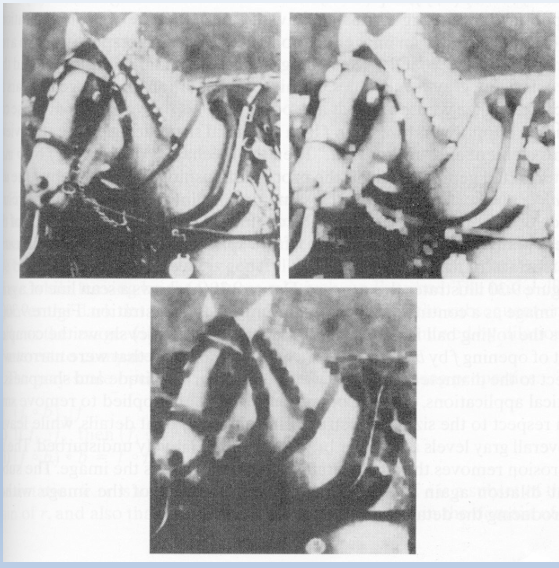
\includegraphics[width=0.6\textwidth]{images/31_1.png}
		\caption{Grayscale erosion trên ảnh con ngựa}
		\label{fig:erosion_horse}
	\end{figure}
	
	\textbf{Giải thích:}
	\begin{itemize}
		\item Hình trên bên trái: ảnh gốc ban đầu.
		\item Hình trên bên phải: kết quả sau khi áp dụng grayscale erosion.
		\item Hình dưới: cho thấy độ tương phản ở các chi tiết nhỏ bị giảm rõ rệt.
		\item Các cạnh sáng bị mòn đi, đặc biệt ở dây cương ngựa, do vùng sáng bị làm tối đi.
		\item Hiệu ứng tổng thể là làm sắc nét hơn các vùng tối, thu gọn kích thước các vùng sáng.
	\end{itemize}
	
	\subsection{Hình 2: Grayscale erosion loại bỏ nhiễu}
	
	\begin{figure}[h!]
		\centering
		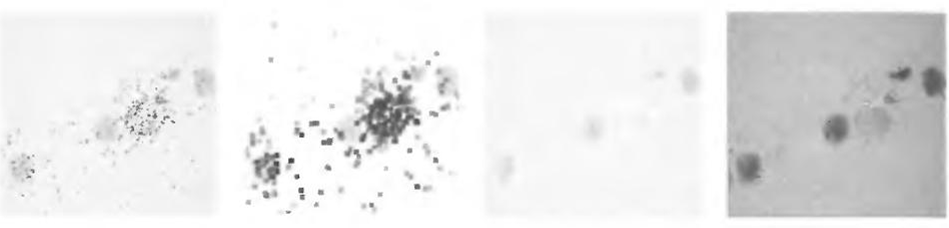
\includegraphics[width=0.9\textwidth]{images/31_2.png}
		\caption{Grayscale erosion loại bỏ nhiễu và giữ lại các vùng tối lớn}
		\label{fig:erosion_dots}
	\end{figure}
	
	\textbf{Giải thích:}
	\begin{itemize}
		\item Dãy ảnh từ trái sang phải thể hiện tác dụng của erosion theo thời gian hoặc khi tăng kích thước phần tử cấu trúc.
		\item Các nhiễu nhỏ, pixel tối lẻ tẻ bị loại bỏ dần do không đủ lớn để giữ lại.
		\item Chỉ còn lại các cụm điểm tối thực sự có kích thước đáng kể (ví dụ: vết tròn đen ở hình bên phải).
		\item Đây là bước tiền xử lý tốt trong các ứng dụng phát hiện vết bệnh, lỗi ảnh, hoặc chuẩn bị cho phân đoạn.
	\end{itemize}
	
	
	
\end{document}